%
% Documento: Trabalhos Relacionados
%
\chapter{Uso do modelo}

Por se tratar de uma extensão da classe \verb|abntex2|, todas as opções, ambientes e macros da classe \verb|abntex2|\cite{abntex2classe}
e \verb|memoir|\cite{madsen2021memoir} podem ser utilizadas.


\section{Opções para a classe \texttt{ifrjtex}}

As opções \verb|artigo| e \verb|projeto| podem ser passadas ao carregar a classe para que a folha de rosto seja ajustada automaticamente ao formato exigido pelo Manual de Apresentação de Trabalhos Acadêmicos \cite{ifrjtccs}.

Caso o usuário opte por editar estes elementos, recomendamos que seja redefinida as macros específicas para a impressão dos mesmos fornecidas pela \verb|abntex2|\cite{abntex2classe}.

\subsection{Projetos de Pesquisa}
Conforme definido no Manual de Apresentação de Trabalhos Acadêmicos, a estrutura de um projeto podem variar conforme as normas estabelecidas pela instituição.
\begin{citacao}
O projeto de pesquisa é um planejamento das etapas do trabalho que será desenvolvido. Sua estrutura pode variar de acordo com as normas estabelecidas pela instituição, sendo constituído pela parte externa e pela parte interna. A externa constitui-se de capa (obrigatória), e a interna é organizada por elementos pré-textuais, elementos textuais e elementos pós-textuais.\cite{ifrjtccs}
\end{citacao}

Para que o modelo imprima os elementos pré-textuais com os elementos exigidos no Manual, a opção \verb|projeto| pode ser passada à classe quando a mesma for selecionada, conforme segue.

\textbackslash\texttt{documentclass[projeto]\{ifrjtex\}}

No entanto, ao construir este modelo em \LaTeX, o autor disponibilizou, além dos elementos exigidos, a macro \verb|\areaconcentracao{}|, visto que muitos programas podem exigir entregas de projetos vinculados à áreas de concentração ou linhas de pesquisa, por exemplo. Dessa forma, optou-se por imprimir na folha de rosto a entrada da macro \verb|\areaconcentracao{}| caso esta seja preenchida.

Os dados da macro \verb|\areaconcentracao{}| são impressos por padrão na folha de rosto após o preâmbulo com o rótulo ``\textbf{Área de concentração: }''.

Caso o usuário queira modificar esse rótulo, pode-se passar um novo rótulo como opção para a macro \verb|\areaconcentracao{}|. Por exemplo, se no preâmbulo o usuário substituir \verb|\areaconcentracao{Nome da área de concentração}| por \\ \verb|\areaconcentracao[Linha de pesquisa: ]{Nome da linha}|, será impresso o rótulo ``\textbf{Linha de pesquisa: }'' no lugar de ``\textbf{Área de concentração: }''.

\subsection{Artigos}
Segundo orientações do Manual de Apresentação de Trabalhos Acadêmicos
\begin{citacao}
Os autores dos artigos submetidos em periódicos externos e de acesso livre, que utilizaram esse tipo de publicação como TCC, deverão comunicar à
Biblioteca do campus onde cursaram sobre a existência da pesquisa, enviando uma cópia do artigo para depósito no repositório institucional (RI) do IFRJ, observando a obrigatoriedade da utilização dos seguintes elementos pré- textuais:\\
    a) capa: elemento obrigatório, deverá ser feita conforme o modelo no Apêndice A e o especificado na seção 2.1;\\
    b) folha de rosto: elemento obrigatório, contém os elementos essenciais à identificação do artigo, de acordo com Apêndice E;\\
   c)verso da folha de rosto: elemento obrigatório, contém a ficha catalográfica confeccionada obrigatoriamente por um bibliotecário da Instituição;\\
    d)folha de aprovação: elemento obrigatório, contém os elementos essenciais à aprovação do trabalho. Após a assinatura da banca, a folha deve ser digitalizada e inserida no documento digital. \cite{ifrjtccs}
\end{citacao}

Para que o modelo imprima esses elementos em conformidade com o Manual, a opção \verb|artigo| pode ser passada à classe quando a mesma for selecionada, conforme segue.

\textbackslash\texttt{documentclass[artigo]\{ifrjtex\}}

Para inserção do artigo submetido em periódicos externos e de acesso livre, recomendamos que o autor utilize após a folha de aprovação o comando \\ \noindent\verb|\includepdf[pages=-]{myfile.pdf}| fornecido pelo pacote \verb|pdfpages| \cite{pdfpages}.




\section{Referências bibliográficas e citações}

Nesta versão da classe, optamos por utilizar o tratamento das referências bibliográficas com o {\ttfamily biblatex} e o estilo \texttt{abnt}, visto que
\begin{citacao}
Sendo totalmente implementado em \LaTeX, ele substitui os arquivos de estilo \verb|bibtex abntex2-alf.bst, abntex2-num.bst| e o pacote \verb|abntex2cite.sty| descrito neste manual. Com isso, o \verb|biblatex-abnt| deve aposentar os estilos de formatação do \verb|abntex2cite| e utilizar exclusivamente o \verb|biblatex-abnt| e as macros padrões do Bib\LaTeX. \cite{araujopacote}
\end{citacao}

Recomendamos que seja lida as referências específicas dos pacotes \verb|biblatex-abnt| disponíveis em \url{https://www.ctan.org/pkg/biblatex-abnt}.

Conforme orientado por \textcite{marquesbiblatex}, o \verb|biblatex-abnt 3.4| requer \verb|biblatex 3.8| e \verb|biber 2.8| e caso haja algum problema na compilação, cheque se seus pacotes estão atualizados.

Exemplos de entrada para o \verb|biblatex|, semelhantes aos encontrados no arquivo \verb|refbase.bib| deste projeto, podem ser encontradas em \textcite{marquesbiblatex} e todas as possíveis entradas, distinguindo entre campos obrigatórios e opcionais podem ser consultadas em \cite{lehman2006biblatex}. Além disso, todas as saídas geradas conforme a NBR 10520:2002 usando o sistema autor-data podem ser consultadas em \textcite{marquesexemplos}.

Recomenda-se ainda que o potencial usuário deste modelo utilize gerenciadores de bases bibliográficas como o \textcite{JabRef2009} e \textcite{Zotero}.

\subsection{Citações livres}\label{citacoesLivres}
Citações são trechos transcritos ou informações retiradas das publicações consultadas para a realização do trabalho.
As citações são utilizadas no texto com o propósito de esclarecer, completar, embasar ou corroborar as ideias do autor.

Todas as publicações consultadas e efetivamente utilizadas (através de citações) devem ser listadas, obrigatoriamente, nas referências bibliográficas, de forma a preservar os direitos autorais e intelectuais.

Na utilização de citações, normalmente, utiliza-se referências.
Para cada tipo de referência presente no texto será apresentado um exemplo do comando utilizado para criá-lo.

Há basicamente dois tipos de citações: citações livres e citações literais.

Nas citações livres, reproduzem-se as ideias e informações de um autor, sem, entretanto, ``copiar letra por letra'' o texto do autor.
Há várias maneiras de se fazer uma citação livre, como mostra os exemplos abaixo.

Por outro lado, \textcite{maturana:2003} defende um princípio de lógica.
Para o autor, quando dizemos \ldots

Além disso, \textcite{teste:2004} argumenta que \ldots\mbox{ }Observe o detalhe do termo \textit{et al}.
que deve ser utilizado quando o trabalho citado possui mais de três autores.
Esse recurso é automatizado pelo estilo {\ttfamily abntex2}\index{ABNT!abntex2}.
Caso não haja desejo em abreviar o nome dos demais autores através do termo \textit{et al.}, deve-se incluir a opção {\ttfamily abnt-no-etal-label}.

Para evitar uma interrupção na sequência do texto, o que poderia, eventualmente, prejudicar a leitura, pode-se indicar a fonte entre parênteses imediatamente após a citação livre.
Porém, neste caso específico, o nome do autor deve vir em caixa alta, seguido do ano da publicação, como no exemplo a seguir.

\cite{BibTeX2009}

\subsection{Citações literais}\label{citacoesLiterais}
Nas citações literais, reproduzem-se as ideias e informações de um autor, exatamente como este a expressou, ou seja, faz-se uma ``cópia letra por letra'' do texto do autor.
Há várias maneiras de se fazer uma citação literal, como mostra os exemplos abaixo.

As citações longas (mais de 3 linhas) devem usar um parágrafo específico para ela, na forma de um texto recuado (4 cm da margem esquerda), com tamanho de letra menor do aquela utilizada no texto e espaçamento simples entre as linhas, seguido dos sobrenomes dos autores em caixa alta (separados por ponto e vírgula), ano de publicação e número da página.
Veja o exemplo abaixo.

\begin{citacao}
Desse modo, opera-se uma ruptura decisiva entre a reflexividade filosófica, isto é a possibilidade do sujeito de pensar e de refletir, e a objetividade científica.
Encontramo-nos num ponto em que o conhecimento científico está sem consciência.
Sem consciência moral, sem consciência reflexiva e também subjetiva.
Cada vez mais o desenvolvimento extraordinário do conhecimento científico vai tornar menos praticável a própria possibilidade de reflexão do sujeito sobre a sua pesquisa \cite[p.28]{morinmoigne:2000}.
\end{citacao}

Para se criar o efeito demonstrado na citação anterior, deve-se utilizar o ambiente \texttt{citacao}.
\begin{verbatim}
\begin{citacao}
    Desse modo, opera-se uma ruptura decisiva entre a reflexividade
    filosófica, isto é a possibilidade do sujeito de pensar e de refletir,
    e a objetividade científica. Encontramo-nos num ponto em que o 
    conhecimento científico está sem consciência.
    Sem consciência moral, sem consciência reflexiva e também subjetiva.
    Cada vez mais o desenvolvimento extraordinário do conhecimento 
    científico vai tornar menos praticável a própria possibilidade 
    de reflexão do sujeito sobre a sua pesquisa \cite[p.28]{morinmoigne:2000}.
\end{citacao}
\end{verbatim}

Opcionalmente, pode-se referenciar os autores no corpo de texto (neste caso seus nomes devem vir em minúsculas), e em seguida colocar a citação literal, em um novo parágrafo recuado.
Note que pode após a citação literal não mais aparece o nome dos autores, visto que já se encontra no texto.
Veja o exemplo seguinte.

\textcite[p.~33]{morinmoigne:2000}, ao fazerem as suas críticas à ciência, explicitam uma ideia coletiva:

\begin{citacao}
Mas o curioso é que o conhecimento científico que descobriu os meios realmente extraordinários para, por exemplo, ver aquilo que se passa no nosso sol, para tentar conceber a estrutura das estrelas extremamente distantes, e até mesmo para tentar pesar o universo, o que é algo de extrema utilidade, o conhecimento científico que multiplicou seus meios de observação e de concepção do universo, dos objetos, está completamente cego, se quiser considerar-se apenas a si próprio!
\end{citacao}

As citações curtas (menos de 3 linhas) devem ser inseridas diretamente no texto (entre aspas), seguida do nome do autor (em caixa alta), ano e página, como no exemplo a seguir.

Então significa apenas que ``assumo que não posso fazer referência a entidades independentes de mim para construir meu explicar'' \cite[p.~35]{maturana:2003}.

O conhecimento de \textcite[p.~35]{maturana:2003} aponta que isto significa apenas que ``assumo que não posso fazer referência a entidades independentes de mim para construir meu explicar''.

Finalmente, e isto vale para citações curtas ou longas, caso seja necessário inserir, no meio de uma citação uma palavra ou frase curta de sua autoria, que sirva para clarear ou completar a frase do autor citado, isto deve ser feito colocando a citação entre aspas.
O comentário deverá ser inserido sem aspas.
Ou seja, todo texto da citação deverá ficar envolvido por aspas.
O exemplo abaixo apresenta o resultado esperado.

Significa apenas que ``assumo que não posso fazer referência a entidades'' objetivas no sentido tradicional ``independentes de mim para construir meu explicar'' {\textcite[p.~35]{maturana:2003}}.

\subsection{Comandos para citações}\label{referenciasUtilizadas}

Alguns exemplos de citação conforme \textcite{marquesbiblatex}:

\begin{itemize}
    \item \textcite{maturana:2003}\\ \verb|\textcite{maturana:2003}|
    \item \textcite{teste:2004}\\ \verb|\textcite{teste:2004}|
    \item \cite[p.~28]{morinmoigne:2000}\\ \verb|\cite[p.~28]{morinmoigne:2000}|
    \item \textcite[p.~33]{morinmoigne:2000}\\ \verb|\textcite[p.~33]{morinmoigne:2000}|
    \item \cite[p.~35]{maturana:2003}\\ \verb|\cite[p.~35]{maturana:2003}|
    \item \textcite[p.~35]{maturana:2003}\\ \verb|\textcite[p.~35]{maturana:2003}|
    \item \cite{teste:2004,maturana:2003}\\ \verb|\cite{teste:2004,maturana:2003}|
    \item \apud{maturana:2003}{morinmoigne:2000}\\
    \verb|\apud{maturana:2003}{morinmoigne:2000}|
\end{itemize}


%
% Documento: Fundamentação Teórica
%

\chapter{Elementos flutuantes, equações e referências cruzadas}
\label{chap:ef}

\textcolor{red}{\large ESTE CAPÍTULO SERÁ ATUALIZADO COM ORIENTAÇÕES DE USO DE MELHORES PACOTES!!}

A seguir ilustra-se a forma de incluir figuras, tabelas, equações, siglas e 
símbolos no documento, obtendo indexação automática em suas respectivas
                listas.
A numeração sequencial de figuras, tabelas e equações ocorre de modo automático.
Referências cruzadas são obtidas através dos comandos \verb#\label{}# e \verb#\ref{}#.
Por exemplo, não é necessário saber que o número deste capítulo é \ref{chap:ef} para colocar o seu número no texto.
Isto facilita muito a inserção, remoção ou relocação de elementos numerados no texto (fato corriqueiro na escrita e correção de um documento acadêmico) sem a necessidade de renumerá-los todos.





 
\section{Equações}
\label{sec:equacoes}

A transformada de Laplace é dada na \autoref{eq:laplace}, enquanto a \autoref{eq:dft} apresenta a formulação da transformada discreta de Fourier bidimensional\footnote{Deve-se reparar na formatação esteticamente perfeita destas equações.}.


\begin{equation}
    X(s) = \int\limits_{t = -\infty}^{\infty} x(t) \, \text{e}^{-st} \, dt
    \label{eq:laplace}
\end{equation}

\begin{equation}
    F(u, v) = \sum_{m = 0}^{M - 1} \sum_{n = 0}^{N - 1} f(m, n) \exp \left[ -j 2 \pi \left( \frac{u m}{M} + \frac{v n}{N} \right) \right]
    \label{eq:dft}
\end{equation}


\section{Elementos flutuantes (tabelas, quadros, gráficos e figuras)}

Tabelas, quadros, gráficos e figuras são elementos utilizados em trabalhos acadêmicos, e possuem diferenças e especificações definidas pela ABNT.

As tabelas são formadas por linhas verticais, devem manter suas bordas laterais abertas e geralmente são utilizadas para dados quantitativos. Os quadros, por outro lado, são formados por linhas verticais e horizontais, devem ter todas suas extremidades fechadas e são mais utilizados para dados qualitativos.

Por último, as figuras e gráficos são elementos ilustrativos, que podem ser em forma de fotos, mapas, gráficos, gravuras, etc.

Todos estes elementos devem estar centralizados, com legenda na parte superior e fonte na parte inferior (ver Quadro \ref{quadroex1} para maiores detalhes).

De forma geral, esses ambiantes podem ser utilizados com os seguintes comandos



\begin{verbatim}
\begin{nome do ambiente}[H]
   \centering
   \caption{legenda}
   \label{"etiqueta"}
      inserção do elemento 
   \fonte{fonte do elemento}
\end{table}
\end{verbatim}
Os campos apresentados nos códigos acima estão explicados no Quadro \ref{quadroex2}.


\begin{quadro}[H]
	\centering
	\caption{Alguns detalhes sobre elementos flutuantes}
	\label{quadroex1}
	\begin{tabular}{|l|m{4cm}|m{4cm}|m{4cm}|}
		\hline
		& \textbf{Tabela}                                                                             & \textbf{Quadro}                                                                             & \textbf{Figuras}                                                                    \\ \hline
		\textbf{Formato}    & Bordas laterais não podem ser fechadas.                                                     & As extremidades devem ser fechadas.                                                         & Podem ser em forma de fotos, mapas, gráficos, gravuras, etc.                        \\ \hline
		\textbf{Uso}        & Geralmente para dados quantitativos.                                                        & Geralmente para dados qualitativos.                                                         & Ilustrar informações e dados.                                                       \\ \hline
		\textbf{Elementos}  & Título, cabeçalho, conteúdo, fonte e, se necessário, notas explicativas.                    & Título, fonte, legenda e notas.                                                             & Título, numeração e fonte.                                                          \\ \hline
		\textbf{Divisão}    & Formada por linhas verticais.                                                               & Formado por linhas horizontais e verticais.                                                 & -                                                                                   \\ \hline
		\textbf{Formatação} & O número e o título da tabela devem vir acima dela, enquanto a fonte deve aparecer embaixo. & O número e o título do quadro devem vir acima dele, enquanto a fonte deve aparecer embaixo. & O número e o título devem aparecer no topo, enquanto a fonte deve aparecer embaixo. \\ \hline
	\end{tabular}
	\fonte{\textcite{diana}}
\end{quadro}

\begin{quadro}[H]
	\centering
	\caption{Alguns campos utilizados em elementos flutuantes}
	\label{quadroex2}
	\begin{tabular}{|m{4cm}|m{8cm}|}
		\hline
	\verb|nome do ambiente| & \verb|figure|: para figuras, \verb|grafico|: para gráficos, \verb|table|: para tabelas e \verb|quadro|: para quadros\\ \hline
	\verb|legenda| & Deve ser inserida como argumento no comando \verb|\caption{}| e refere-se a legenda do elemento flutuante.\\ \hline
	\verb|"etiqueta"| & Deve ser inserida como argumento no comando \verb|\label{}| e consiste em um nome dado para referenciarmos àquele elemento flutuante no texto.\\ \hline
	\verb|fonte do elemento| & Deve ser inserida como argumento no comando \verb|\fonte{}| e consiste da informação de onde retirou-se o elemento.\\ \hline
	\end{tabular}
	\fonte{Elaborado pelo autor}
\end{quadro}


Abaixo apresentamos alguns exemplos de outros elementos flutuantes  seguidos dos códigos utilizados para inseri-los.

A Figura \ref{fig:conceitodt} aparece automaticamente na lista de figuras.
Para uso avançado de imagens no \LaTeX, recomenda-se a consulta de literatura especializada \cite{Goossens2007}.

\begin{figure}[H]
	\centering
	\caption{Ilustração do conceito de derivada topológica.}
	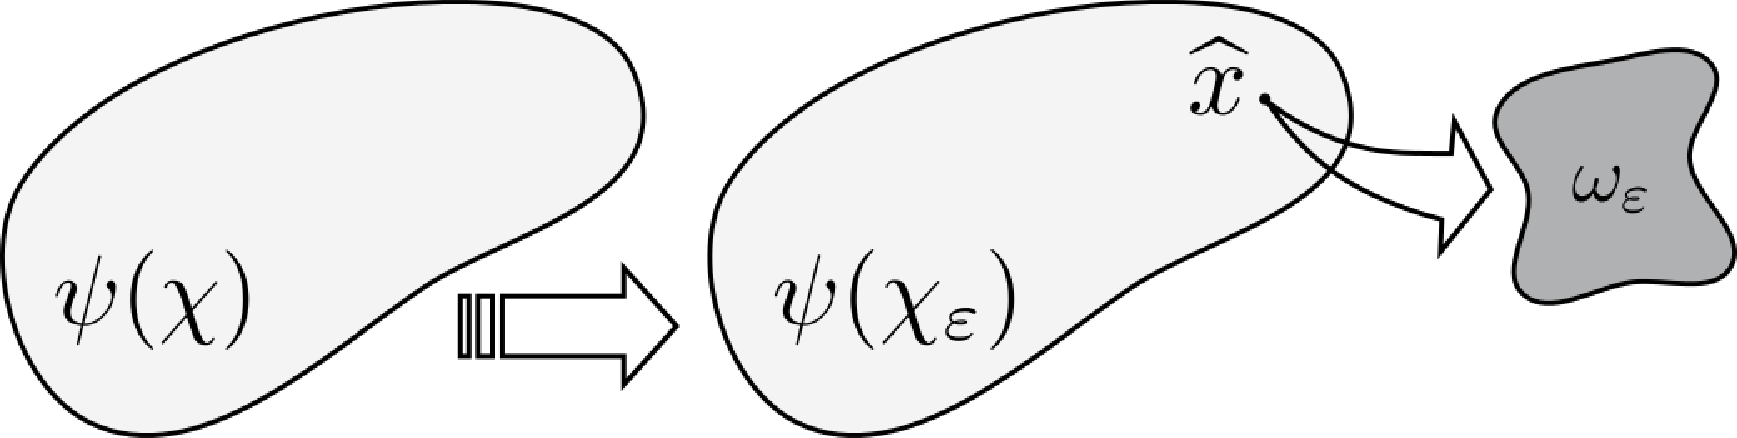
\includegraphics[width=0.6\textwidth]{./figuras/conceito.pdf}
	\fonte{\textcite{NovotnyBook2013}}
	\label{fig:conceitodt}
\end{figure}

\begin{verbatim}
\begin{figure}[H]
  \centering
  \caption{Conceito de derivada topológica.}
    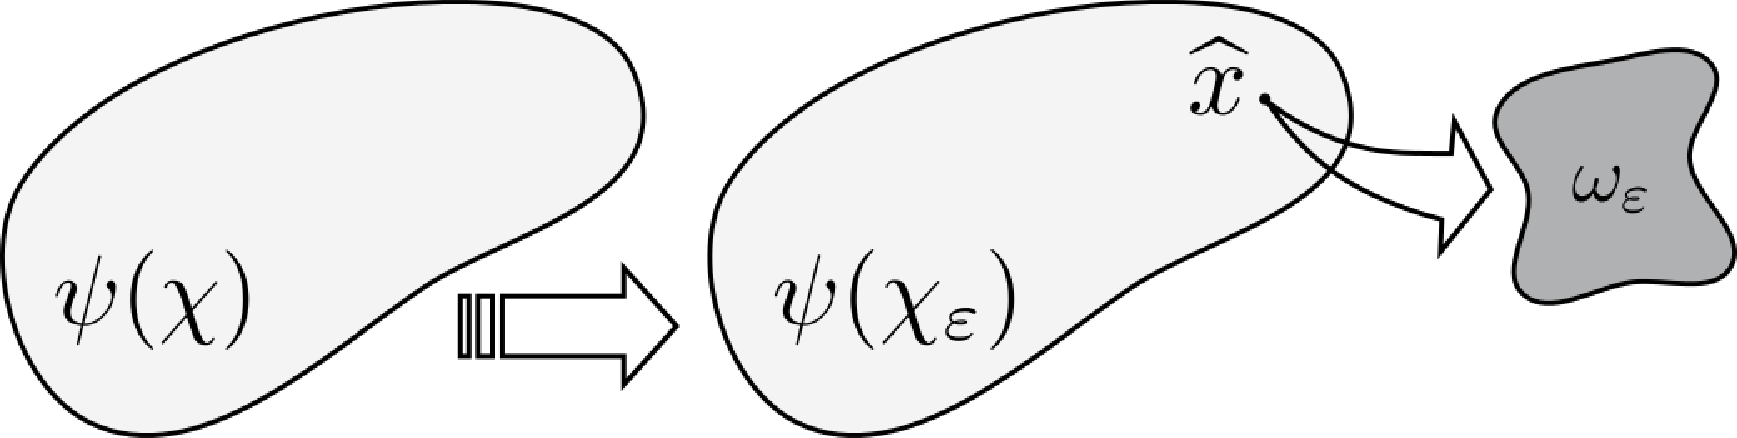
\includegraphics[width=0.6\textwidth]{./figuras/conceito.pdf}
  \fonte{\textcite{NovotnyBook2013}}
  \label{fig:conceitodt}
\end{figure}
\end{verbatim}


\begin{table}[H]
\centering
\caption{Um nome qualquer}
\label{ExemploTab}
\begin{tabular}{r|lr}	
Posição & País & IDH \\ \hline
	1 & Noruega        & .955 \\
	2 & Austrália  & .938 \\
	3 & EUA            & .937 \\
	4 & Holanda        & .921 \\
	5 & Alemanha       & .920            % não é preciso quebrar a última linha
\end{tabular}
% \fonte{\textcite{garcia}}
\end{table}

\begin{verbatim}
\begin{table}[H]
\centering
\caption{Um nome qualquer}
\label{ExemploTab}
\begin{tabular}{r|lr}	
    	Posição & País & IDH \\	\hline
    	1 & Noruega        & .955 \\
    	2 & Austrália  & .938 \\
    	3 & EUA            & .937 \\
    	4 & Holanda        & .921 \\
    	5 & Alemanha       & .920 
\end{tabular}
\fonte{\textcite{garcia}}
\end{table}
\end{verbatim}


\pagebreak

No Gráfico \ref{gr:exgrafico} apresentamos um exemplo de gráfico.

\begin{grafico}[H]
\centering
\caption{Evolução de matrículas dos Institutos Federais}
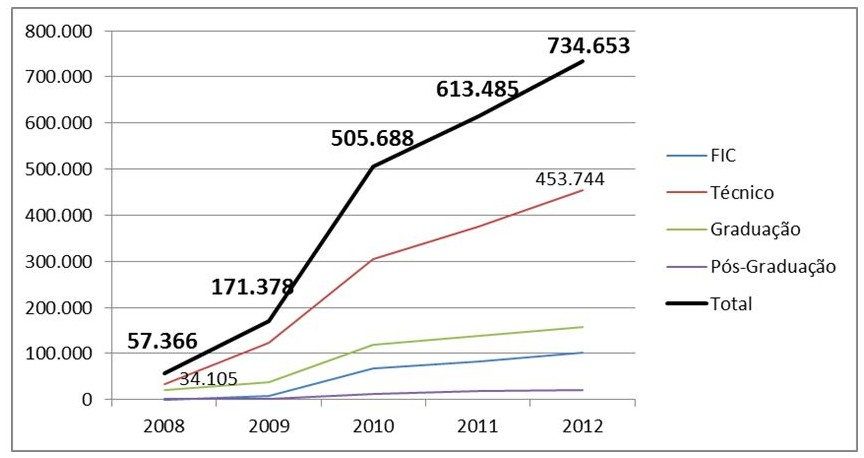
\includegraphics[height=6cm]{./figuras/redefederal.jpg}	
\fonte{MEC/SETEC}
\label{gr:exgrafico}
\end{grafico}

\begin{verbatim}
\begin{grafico}[H]
  \centering
  \caption{Evolução de matrículas dos Institutos Federais}
    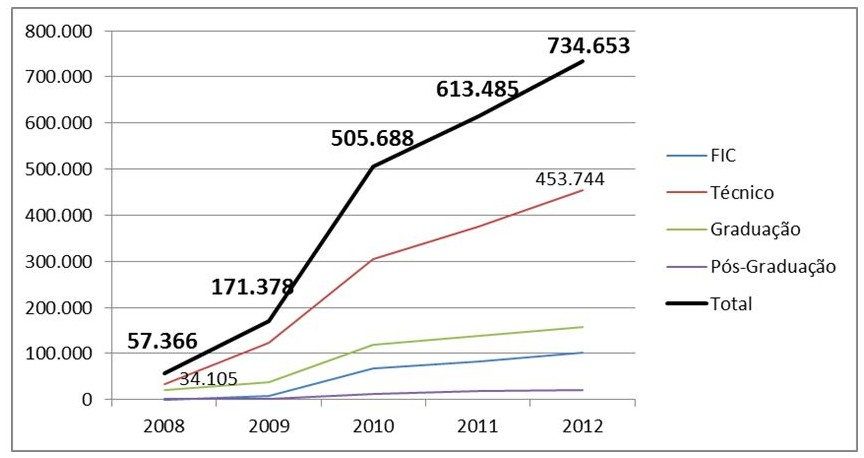
\includegraphics[height=6cm]{./figuras/redefederal.jpg}	
  \fonte{MEC/SETEC}
  \label{gr:exgrafico}
\end{grafico}
\end{verbatim}